\chapter{Einleitung}

\section{Motivation und Problemstellung}

Die digitale Transformation ist ein zentrales Anliegen der deutschen Versicherungswirtschaft. So gaben Versicherungsunternehmen im Jahr 2020 5.6 Milliarden Euro für \ac{it} aus, um bspw. ihre Infrastruktur zu modernisieren, auf Cloud-Lösungen umzustellen und in neue Technologien zu investieren. \autocite[Vgl.][S. 2]{PATRIK2023} In der Versicherungsbranche herrscht zudem ein hoher Wettbewerbsdruck, die Kundenanforderungen steigen ständig, insbesondere im Hinblick auf Serviceangebote und -qualität. Moderne, wechselwillige Kunden möchten rund um die Uhr auf Self-Service-Basis mit ihrem Versicherer kommunizieren, um Angebote zu erhalten, Anträge zu stellen oder Ansprüche geltend zu machen. \autocite[Vgl.][]{SCHMIDT2022} 

Besonders deutlich sind diese Veränderungen in der Kraftfahrzeug-Versicherungs-branche (\acsu{kfz}-Versicherungsbranche) zu erkennen. So ist gemäß einer Studie von Statista aus dem Jahr 2022 die Kfz-Versicherungssparte mit mehr als 26 \% online abgeschlossener Verträge in der deutschen Versicherungsindustrie aktuell führend. \autocite[Vgl.][]{STATISTA2023} 

Bei der Wahl des Versicherungsanbieters stehen dabei vor allen Dingen die Einfachheit und Klarheit der Versicherungsleistung, sowie die Anpassungsmöglichkeit der Versicherung an das eigene Fahrverhalten und individuelle Bedürfnisse im Vordergrund. Zudem kommen der Vergleichbarkeit von Leistungen und der wettbewerbsfähigen Preisgestaltung aufgrund der hohen Markttransparenz eine große Bedeutung zu. \autocite[Vgl.][]{MITZNER2023} So haben in Deutschland 2022 29 \% der Versicherungsnehmer ihren Kfz-Versicherungsanbieter gewechselt. \autocite[Vgl.][]{ASSCOMPACTNEWSFURASSEKURANZUNDFINANZWIRTSCHAFT2023} 

Eine zentrale Ursache hierfür ist der mangelnde Kundenkontakt, weshalb es laut dem Vertriebsvorstand der Neodigital Versicherung AG Stephen Voss umso wichtiger ist, dass die wenigen Kontaktpunkte einfach, schnell und praktisch ablaufen, damit der Versicherungsanbieter vom Kunden nicht negativ wahrgenommen wird. Folglich ist es für die Kfz-Versicherer wichtig, ihren digitalen Auftritt zu verbessern und dem Kunden innovative Produkte sowie benutzerfreundliche Services bereitzustellen. \autocite[Vgl.][]{VOSS2022}

%Eine zentrale Ursache hierfür ist der mangelnde Kundenkontakt und die daraus resultierende niedrige Kundenloyalität. Daher ist es laut dem Vertriebsvorstand der Neodigital Versicherung AG Stephen Voss umso wichtiger, dass die wenigen Kontaktpunkte einfach, schnell und praktisch ablaufen, sodass der Versicherungsanbieter vom Kunden nicht negativ wahrgenommen wird. Für die Versicherer ist es deshalb wichtig, ihren digitalen Auftritt zu verbessern und dem Kunden innovative, Produkte sowie benutzerfreundliche Services bereitzustellen. \autocite[Vgl.][]{VOSS2022}

Um die digitale Transformation erfolgreich zu bewältigen, ist nicht eine einzelne Komponente entscheidend, sondern die Kfz-Versicherer benötigen vielmehr eine digitale Plattform, mit der Geschäftsprozesse optimiert, Daten intelligent genutzt und zusätzliche Partner integriert werden können. \autocite[Vgl.][]{WEINGARTNER2023}
% Diese Plattform muss alle erforderlichen technischen Technologien und Services bieten, um Geschäftsprozesse zu digitalisieren, Daten intelligent zu nutzen und zusätzliche Partner zu integrieren. \autocite[Vgl.][]{WEINGARTNER2023}

%Die Digitalisierung ist ein zentrales Anliegen der deutschen Versicherungswirtschaft. Viele Versicherungsunternehmen modernisieren derzeit ihre IT-Infrastrukturen, stellen ihre IT-Landschaft auf Cloud-Lösungen um, investieren in neue Zugangskanäle oder in innovative Technologien um ihren Kunden verbesserte Produkte und Dienstleistungen anzubieten. Im Jahr 2020 gaben Versicherungsunternehmen 5.6 Milliarden Euro für IT aus. Damit gehört diese zu den wesentlichen Investitionsschwerpunkten der Versicherungsunternehmen. \autocite[Vgl.][S. 2]{PATRIK2023}

%In der Versicherungsbranche herrscht zudem ein hoher Wettbewerbsdruck, die Kundenanforderungen steigen ständig, insbesondere im Hinblick auf Serviceangebote und -qualität. Moderne, wechselwillige Kunden möchten rund um die Uhr auf Self-Service-Basis mit ihrem Versicherer kommunizieren, um Angebote zu erhalten, Anträge zu stellen oder Ansprüche geltend zu machen. \autocite[Vgl.][]{SCHMIDT2022} 

%Besonders deutlich sind diese Veränderungen in der Kfz-Versicherungsbranche zu erkennen. So ist gemäß einer Studie von Statista aus dem Jahr 2022 die Kfz-Versicherungssparte mit mehr als 26 \% online abgeschlossener Verträge in der deutschen Versicherungsindustrie aktuell führend. \autocite[Vgl.][]{STATISTA2023} 

%Bei der Wahl des Versicherungsanbieters stehen dabei vor allem die Einfachheit und Klarheit der Versicherungsleistung, die Anpassungsmöglichkeit der Versicherung an das eigene Fahrverhalten sowie individuelle Bedürfnisse im Vordergrund. Der Vergleichbarkeit von Leistungen und der wettbewerbsfähigen Preisgestaltung kommt durch die große Markttransparenz zusätzlich eine hohe Bedeutung zu.\autocite[Vgl.][]{MITZNER2023} So haben bei sehr ähnlichen Produkten in Deutschland 2022 29 \% der Versicherungsnehmer ihren Kfz-Versicherungsanbieter gewechselt. \autocite[Vgl.][]{ASSCOMPACTNEWSFURASSEKURANZUNDFINANZWIRTSCHAFT2023} 

%Eine Ursache hierfür ist auch im mangelnden Kundenkontakt und der daraus resultierenden niedrigen Kundenloyalität zu finden. Daher ist laut dem Vertriebsvorstand der Neodigital Versicherung AG Stephen Voss umso wichtiger, dass die wenigen Kontaktpunkte einfach, schnell und praktisch ablaufen, sodass der Versicherungsanbieter vom Kunden nicht negativ wahrgenommen wird.\autocite[Vgl.][]{VOSS2022}

%Für die Versicherer ist es deshalb wichtig, ihren digitalen Auftritt zu verbessern und dem Kunden innovative Produkte und benutzerfreundliche Services bereitzustellen. 

%Um die digitale Transformation erfolgreich zu meistern werden, ist nicht eine einzelne Komponente entscheidend, sondern die Kfz-Versicherer benötigen vielmehr eine digitale Plattform. Diese Plattform muss alle erforderlichen technischen Kernprodukte, Technologien und Services bieten, um Geschäftsprozesse zu digitalisieren und optimieren, neue Anwendungen zu integrieren, Daten zu beschaffen, strukturieren und analysieren sowie zusätzliche Partner zu integrieren. (Vgl. WEINGARTNER2023)



%Die digitale Transformation hat tiefgreifende Auswirkungen auf das private sowie das geschäftliche Umfeld und stellt damit auch die eher träge auf Veränderungen reagierende deutsche Versicherungsindustrie vor neue Herausforderungen. Der Wettbewerb in der Branche verschärft sich, während Kunden fortlaufend bessere Serviceangebote und -qualität fordern. Moderne, wechselwillige Kunden möchten mit ihrem Versicherer auf Self-Service-Basis interagieren, um Angebote zu erhalten, Anträge zu stellen oder Ansprüche geltend zu machen. \autocite[Vgl.][]{SCHMIDT2022}

%Besonders deutlich sind diese Veränderungen in der Kraftfahrzeug-Versicherungs-branche (\acsu{kfz}-Versicherungsbranche) zu erkennen. So ist gemäß einer Studie von Statista aus dem Jahr 2022 die \ac{kfz}-Versicherungssparte mit mehr als 26\% online abgeschlossener Verträge in der deutschen Versicherungsindustrie aktuell führend. \autocite[Vgl.][]{STATISTA2023} Bei der Wahl des Anbieters stehen dabei vor allem die Einfachheit und Klarheit der Versicherungsleistung, die Anpassungsmöglichkeiten an das Fahrverhalten sowie der Preis im Vordergrund. \autocite[Vgl.][]{MITZNER2023} Folglich müssen \ac{kfz}-Versicherer ihre internen Prozesse zur Kostenreduktion optimieren und ihren digitalen Auftritt verbessern, um langfristig am Markt wettbewerbsfähig zu sein bzw. zu bleiben. Für diese digitale Transformation ist dabei nicht eine einzelne Komponente entscheidend, sondern die \ac{kfz}-Versicherer benötigen vielmehr eine digitale Plattform, mit der sie eine durchgehende Digitalisierung, Optimierung interner Prozesse sowie eine intelligente Datennutzung erreichen können. \autocite[Vgl.][]{WEINGARTNER2023} 

%\newpage
\section{Zielsetzung und Abgrenzung}

Die SAP \ac{btp} ist eine digitale Plattform, mit der \ac{kfz}-Versicherer ihre bestehende Systemlandschaft transformieren und an neue Geschäftsanforderungen anpassen können.

Ziel dieser Arbeit ist es daher, die Anforderungen der \ac{kfz}-Versicherer an eine digitale Plattform zu identifizieren, um anschließend beurteilen zu können, inwiefern die Anforderungen der \ac{kfz}-Versicherer an eine digitale Plattform von der SAP Business Technology Plattform erfüllt werden. Die aus der Analyse resultierende Handlungsempfehlung soll \ac{kfz}-Versicherern eine praxisorientierte Vorgehensweise zur Nutzung der SAP Business Technology Plattform aufzeigen.

Dabei wird der deutsche \ac{kfz}-Versicherungsmarkt betrachtet, da eine Analyse inklusive internationaler Märkte aufgrund der unterschiedlichen regulatorischen Rahmenbedingungen, divergierender Prämienfaktoren sowie ungleichmäßig ausgeprägter technologischer Fortschritte nicht hinreichend aussagekräftig wäre. Des Weiteren konzentriert sich die Arbeit im Wesentlichen auf die technologischen Merkmale einer digitalen Plattform. 

Darüber hinaus werden im Rahmen dieser Untersuchung digitaler Plattformen als Wettbewerbsfaktor betrachtet, nicht aber in Bezug zu anderen Wettbewerbskräften im Versicherungsmarkt gesetzt.




\section{Aufbau der Arbeit}

Zu Beginn der Projektarbeit werden zunächst digitale Plattformen als disruptive Innovation erläutert. Hierzu werden digitale Plattformen definiert, die Wertschöpfung digitaler Plattformen vorgestellt, Cloud-Computing auf technischen Plattformen beschrieben und darauf aufbauend die SAP Business Technology Platform vorgestellt. Danach werden die Definition und Grundprinzipien der Versicherung sowie der Aufbau und der Wettbewerb in der \ac{kfz}-Versicherungssparte dargestellt. Anschließend wird die Wahl der wissenschaftlichen Methodik begründet und das Vorgehen bei der Task-Technology-Fit-Theorie (\acsu{ttf}-Theorie), der systematischen Literaturanalyse, dem semistrukturierten Leitfadeninterview sowie bei der qualitativen Inhaltsanalyse beschrieben.

\begin{figure}[h]
    \centering
    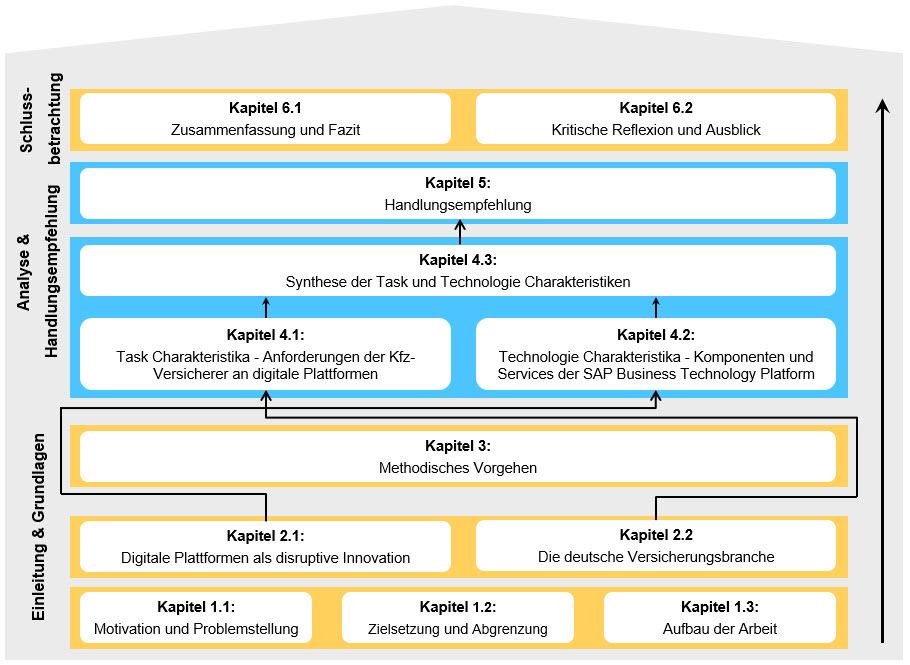
\includegraphics[width=1\textwidth]{img/Aufbau_der_Arbeit2.jpg}
    \caption[Aufbau der Arbeit]{Aufbau der Arbeit\autocite{Aufbau}}
    \label{fig:Aufbau}
\end{figure}
\footnotetext{eigene Darstellung}

Im Anschluss daran werden die Anforderungen der \ac{kfz}-Versicherer an digitale Plattformen mithilfe der systematischen Literaturanalyse identifiziert und anschließend mittels Experteninterviews ergänzt und evaluiert. Daraufhin werden die Funktionalitäten und Services der SAP \ac{btp} vorgestellt, um diese im Anschluss den Anforderungen der \ac{kfz}-Versicherer gegenüberzustellen. Ausgehend von dem Analyseergebnis wird eine Handlungsempfehlung für deutsche \ac{kfz}-Versicherer ausgesprochen. Darauffolgend werden die Vorgehensweise und Analyseergebnisse kritisch reflektiert, um abschließend die Arbeit mit einem Fazit zusammenzufassen und in einem Ausblick mögliche Folgeuntersuchungen aufzuzeigen.(siehe Abbildung \ref{fig:Aufbau})




\newpage